\documentclass{article}

\usepackage[utf8]{inputenc}
\usepackage[spanish]{babel}

\usepackage{caratula}
\usepackage[toc,page]{appendix}
\usepackage{subcaption}
\usepackage{graphicx}
\usepackage{dirtytalk}
\usepackage{enumerate}

\usepackage{amssymb}
\usepackage{mathtools}
\usepackage{amsmath}
\usepackage{amsthm}

\usepackage{algorithm}
\usepackage{algpseudocode}
\usepackage{listingsutf8}

\usepackage{float}
\floatplacement{figure}{h!}

\usepackage{geometry}
\usepackage{fixltx2e}
\usepackage{wrapfig}
\usepackage{cite}
\usepackage{dsfont}
\usepackage{ulem}

\usepackage[space]{grffile}

\geometry{
 a4paper,
 total={210mm,297mm},
 left=30mm,
 right=30mm,
 top=30mm,
 bottom=30mm,
 }
 
\usepackage{booktabs}
 
% sql stuff
\usepackage{listings}
\usepackage{courier}
\usepackage{pdflscape}

\newcommand\JSONnumbervaluestyle{\color{blue}}
\newcommand\JSONstringvaluestyle{\color{red}}

% switch used as state variable
\newif\ifcolonfoundonthisline

\makeatletter

\lstdefinestyle{json}
{
  showstringspaces    = false,
  keywords            = {false,true},
  alsoletter          = 0123456789.,
  morestring          = [s]{"}{"},
  stringstyle         = \ifcolonfoundonthisline\JSONstringvaluestyle\fi,
  MoreSelectCharTable =%
    \lst@DefSaveDef{`:}\colon@json{\processColon@json},
  basicstyle          = \ttfamily,
  keywordstyle        = \ttfamily\bfseries,
}

% flip the switch if a colon is found in Pmode
\newcommand\processColon@json{%
  \colon@json%
  \ifnum\lst@mode=\lst@Pmode%
    \global\colonfoundonthislinetrue%
  \fi
}

\lst@AddToHook{Output}{%
  \ifcolonfoundonthisline%
    \ifnum\lst@mode=\lst@Pmode%
      \def\lst@thestyle{\JSONnumbervaluestyle}%
    \fi
  \fi
  %override by keyword style if a keyword is detected!
  \lsthk@DetectKeywords% 
}

% reset the switch at the end of line
\lst@AddToHook{EOL}%
  {\global\colonfoundonthislinefalse}

\newtheorem{theorem}{Teorema}[section]
\newtheorem{corollary}{Corolario}[theorem]
\newtheorem{lemma}{Lema}[theorem]
 
\theoremstyle{definition}
\newtheorem{definition}{Definición}[section]
 
\theoremstyle{remark}
\newtheorem*{remark}{Observación}

\usepackage[dvipsnames]{xcolor}
 
\begin{document}
% Estos comandos deben ir antes del \maketitle
\materia{Ingeniería de Software II} % obligatorio

\titulo{TP2}
\subtitulo{Alerta y Vigliancia de Yacimientos Semi-Automatico \\ \textbf{AVYSA} \\ \today}
\grupo{}

\integrante{Christian Cuneo}{755/13}{chriscuneo93@gmail.com}
\integrante{Federico Beuter}{827/13}{federicobeuter@gmail.com}
\integrante{Mauro Cherubini}{835/13}{cheru.mf@gmail.com}
\integrante{Mario Ezequiel Ginsberg}{145/14}{ezequielginsberg@gmail.com}
\integrante{Martin Baigorria}{575/14}{martinbaigorria@gmail.com}
 
\maketitle

\tableofcontents

\pagebreak

\section{Casos de uso}

\subsection{Diagrama}

\subsection{Descripcion}

\subsection{Especificacion}

En esta seccion identificaremos los tres casos de uso principales y los especificaremos en detalle utilizando la tabla de curso normal/alternativo.

\pagebreak

\section{Atributos de calidad}

\pagebreak

\section{Arquitectura}

\subsection{Diagrama general}

\begin{figure}[H]
	\resizebox{\textwidth}{!}{
		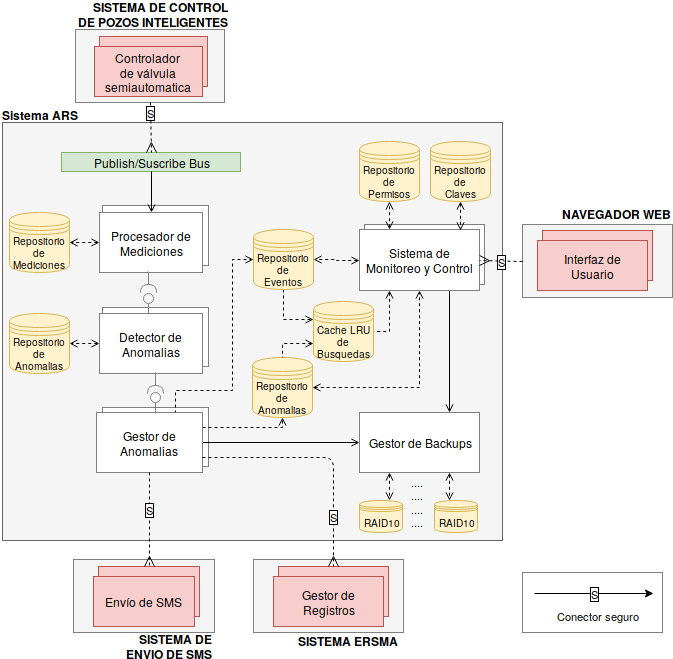
\includegraphics[scale=0.8]{figures/architecture.png}
	}	
	\caption{Diagrama general de la arquitectura del sistema ARS de supervision automatica de yacimientos.}
\end{figure}

\subsection{Procesamiento de mediciones}

\begin{figure}[H]
	\resizebox{\textwidth}{!}{
		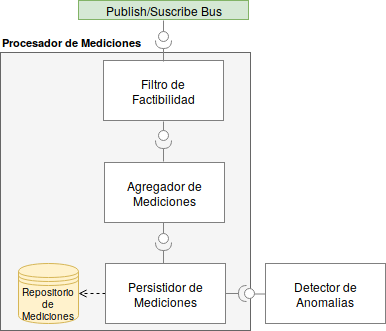
\includegraphics[scale=0.8]{figures/ProcesadorDeMediciones.png}
	}	
	\caption{Diagrama de arquitectura de procesamiento de mediciones.}
\end{figure}

\subsection{Detector de anomalias}

\begin{figure}[H]
	\resizebox{\textwidth}{!}{
		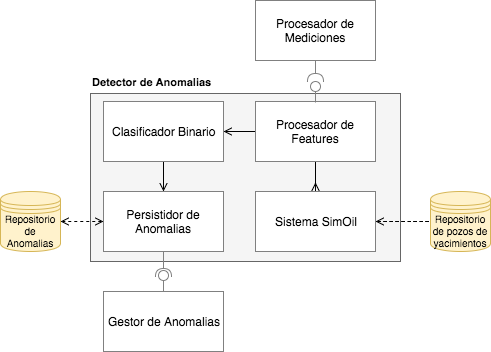
\includegraphics[scale=0.8]{figures/DetectorDeAnomalias.png}
	}	
	\caption{Diagrama de arquitectura del detector de anomalias.}
\end{figure}

\subsection{Gestor de anomalias}

\begin{figure}[H]
	\resizebox{\textwidth}{!}{
		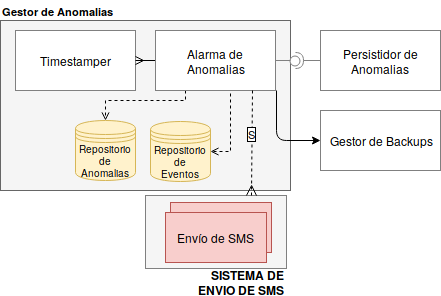
\includegraphics[scale=0.8]{figures/GestorDeAnomalias.png}
	}	
	\caption{Diagrama de arquitectura del gestor de mediciones.}
\end{figure}


\end{document}